\documentclass[10pt,a4paper]{ctexart}
\usepackage[utf8]{inputenc}
\usepackage{amsmath}
\usepackage{amsfonts}
\usepackage{amssymb}
\usepackage{graphicx}
\usepackage{xcolor}
\usepackage{bm}
\author{吴秉哲}
\title{数值分析上机报告}
\begin{document}
\maketitle
这学期每次的上机报告都按如下格式编写:

每份报告分为几个章节,每个章节分别介绍上机作业中的一题,其中每个
题目又分为以下几个部分:
\begin{enumerate}
\item 问题提出及相关背景知识
\item 问题的理论分析及解决方案
\item 程序的部分设计思路与细节
\item 计算成果与分析
\item 本次上机的反思
\end{enumerate}
每个题目中要求回答的问题均蕴含在问题的理论分析与计算成果分析两部分

在程序方面,都是由C++编写完成(其中用到了自己编写的库:矩阵(Matrix),向量(Vector),以及数值代数的相关算法(linear)),在linux下由g++编译。数据方面
一般使用matlab可视化处理,少部分使用了python。

\section{第五章第一题}
\subsection{问题提出及相关背景知识}
题目给出一个严格对家占优的循环矩阵,要求对$N=2^{10}$用FFT的方法解对应的方程组,并与共轭梯度法比较。
\subsection{问题的理论分析及解决方案}
由于所解方程的系数矩阵为严格对家占优的循环矩阵,则可以推导出其为正定对称矩阵,进而可以使用PCG(预优共轭梯度法)进行数值求解。
又由于其为循环矩阵,由教材的推导,可以使用离散傅立叶变化求解,当矩阵的阶数$N=2^n$时,还可以使用FFT加速。

在本题的上机中,直接选取对角矩阵为预优矩阵。
\subsection{程序设计的思路与细节}
本次上机程序设计的主要难点为FFT算法的实现,我在程序中使用了递归来实现FFT。值得一提FFT的算法可以有两种思路,一种为教材的思路,
还有一种从信号处理的角度来看,可以对所变化向量从频域上划分,也可以作类似的实现。我在我的程序Fourier.h中,对这两种方法都有实现。
\subsection{计算成果与分析}
首先给出题目要求的几个特殊结果,然后列出进一步实验的一些数据,最后对两种方法进行分析。

取$N=2^{10}$时,用FFT解对应方程组所得到的结果达到了机器精度,花费了0.006s。取$N=100,N=150$时,PCG法均在迭代8步以内得到了机器精度
的解,所花费的时间分别为

下面我们看一看进一步的结果

不难看出所求方程组的精确解为$(0.5,0.5,\cdots,0.5)^T$,而进行实验方法都可以在一定条件下达到机器精度,于是我主要通过控制相同精度,然后

取$2^{n},n=1,2,\cdots,10$为系数矩阵的阶数,观察两种方法所需要的时间,并将其做可视化处理得到了下面一张图表:
\par
\centerline{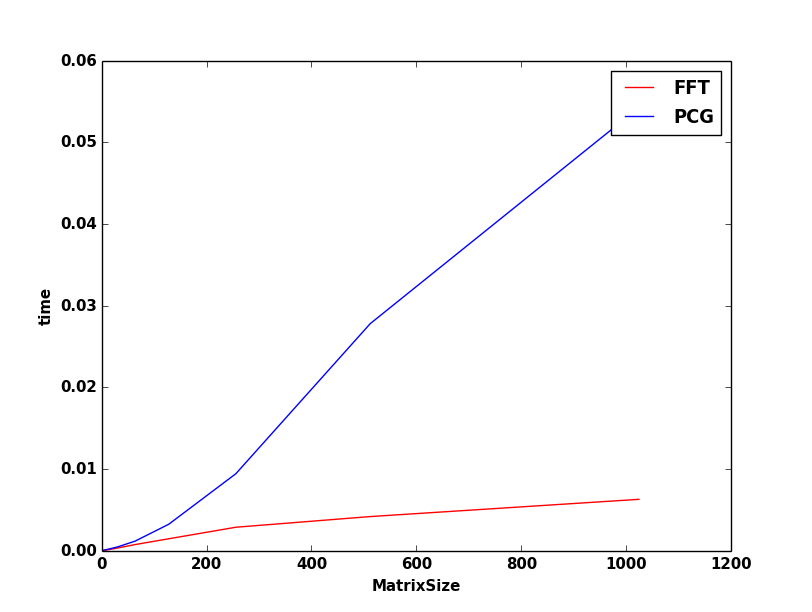
\includegraphics[height=7cm,width=10cm]{fft1.png}}
\par
\subsection{本次上机反思}
\end{document}
